%
% File acl2014.tex
%
% Contact: giovanni.colavizza@epfl.ch
%%
%% Based on the style files for ACL-2013, which were, in turn,
%% Based on the style files for ACL-2012, which were, in turn,
%% based on the style files for ACL-2011, which were, in turn, 
%% based on the style files for ACL-2010, which were, in turn, 
%% based on the style files for ACL-IJCNLP-2009, which were, in turn,
%% based on the style files for EACL-2009 and IJCNLP-2008...

%% Based on the style files for EACL 2006 by 
%%e.agirre@ehu.es or Sergi.Balari@uab.es
%% and that of ACL 08 by Joakim Nivre and Noah Smith

\documentclass[11pt]{article}
\usepackage{acl2014}
\usepackage{times}
\usepackage{url}
\usepackage{latexsym}
\usepackage{multicol}
\usepackage{graphicx}

%\setlength\titlebox{5cm}

% You can expand the titlebox if you need extra space
% to show all the authors. Please do not make the titlebox
% smaller than 5cm (the original size); we will check this
% in the camera-ready version and ask you to change it back.


\title{Song offensiveness vs time and popularity}

\author{Lars Klein \\
  {\tt privatlarsklein@gmail.com} \\\And
  Ahmed Kulovic \\
  {\tt ahmed.kulovic@epfl.ch} \\\And
Ali Hosseiny \\
{\tt ali.hosseiny@epfl.ch} \\}

\date{}

\begin{document}
\maketitle
\begin{abstract}
  This document contains the instructions for preparing a report for ADA 2017. The document itself conforms to its own specifications, and is therefore an example of
  what your manuscript should look like. This document is based on the ACL 2014 paper format.
\end{abstract}



\section{Introduction}

\section{Analysis}

\subsection{Basic correlations}

The first task was to check whether there is a general correlation between the offensiveness (the number of offensive words) and the popularity of a song. Our results are shown on figure \ref{basic_correlations}. We see that the wanted correlations, i.e. the offensiveness-hotness and the offensiveness-counts (play counts) are close to zero so there is no linear dependency if we take all valid songs (those where the play count is greater than 1 and the year is known) into account.

\begin{figure*}

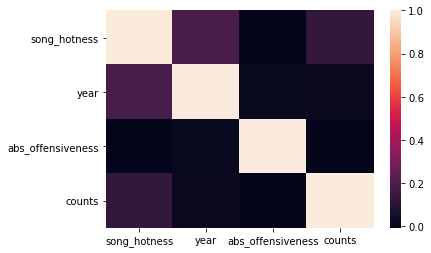
\includegraphics{plots/basic_correlations}
\caption{Basic correlations for all songs}
\label{basic_correlations}
\end{figure*}

We have also tried many different ways to find correlations in our data: 

\begin{itemize}
\item we have tried using the logarithm of the play count instead of the original number of times the songs have been played. This was because the songs which were played often could have a huge value as compared to the ones which were played only 1, 2, 3, or a few times. We wanted to smooth those values so that the difference between popular and non popular songs can be better measured. Unfortunately this didn't give us better correlations than before. However we notice that the correlation between song hotness and play counts suddenly jumped from 0.13 to 0.51 so, at least, we got some insights about the way the song hotness was computed in the Million Songs dataset: they probably also used the logarithm of the play counts value as one of the measures of popularity.
\item We removed songs where the play count was very low hoping that the data was better for more popular songs. So we took only songs that were played at least 4 times. Unfortunately, we still didn't get any improvement out of this.
\item In the same spirit as the previous one we tried to keep only recent songs (we tried both with songs which were released after 1990 and those which were released after 2000). We hoped that the data was better for recent songs and that we could get some meaningful correlations with this strategy, but nothing: the correlations are still close to zero.
 \end{itemize}


\subsection{Correlations over time}

\subsection{Data visualization}

\subsection{Ratio experiment}

\subsection{Number of swear words experiment}

\subsection{Machine learning experiment}


\section{Outview}
In this section we will look at what we could have done differently but didn’t do simply because it was
too complicated or it didn’t make a lot of sense.

\subsection{The hotness problem}
In our dataset we have this hotness (« hotttnesss ») attribute for each song which is
supposed to be a measure of popularity. However, a lot of songs have a hotness equal to 0 or NaN, which
makes our final dataset smaller. But another problem is that we don’t really know how this parameter was
generated. In our analysis we simply trusted it without being sure how it is calculated.
so we tried to come up with other ways of calculating the popularity of songs :

\subsubsection{Youtube}
The main problem is that Youtube was founded in 2005 so we would have no data for music before that
year. This would leave us with a lot of songs we can’t even talk about. And, since one of the core ideas of
our project is to do our analysis based on time (compute the correlations between offensiveness and
popularity over time), this would have left us with only a few years between 2005 and 2010 (the data
stops at 2011), which is probably not enough to do get interesting data. Another issue tightly related to
this one is that the popularity of Youtube itself is variable. For example « Despacito » is the most viewed
video on Youtube today with over 4.5 billion views but, 7 years ago, it was Justin Bieber’s « Baby » with
only 1.7 billion views. It’s probably not that « Despacito » is 2.6 times more popular than « Baby » was
but just that Youtube was not used as much as it is used today. A lot less people had a connection to the
Internet and there were also other means of listening to music (there are also other means today but they
are not the same as before). Simply said, there is a variable we might call « Youtube usage » (or poularity
or acces – you can call it however you want) which varies over time and we would have to scale the
number of views according to this variable, which is quite difficult or maybe even non feasible.


One other problem is the way data is structured on Youtube. The way we would gather our info would be
to simply try to match the names of our songs with the name on Youtube since the track id used in the
Million Songs dataset simply doesn’t exist on Youtube. But, however, we know there can be many videos
for one song. We often have the official video and additional videos with lyrics posted by fans (and there
can be many of them). So the total number of views is scattered all around and we have no way to find a
guarantee that what we are scraping is enough. We might take only official videos but even that is not
such a good idea because we would probably lose a lot of info and we would also fall for fake official
videos. And the view count is not a good measure because a video can be removed and reuploaded
because of artist rights or other things.

\subsubsection{Spotify}
One other idea we had in mind was to use the Spotify API. Spotify is one of the most
popular apps today for listening to music so it can probably be used to gather interesting information. The
Spotify API is very complete since it provides us with all the values we would need in our analysis,
especially with the track info such as play counts for users or popularity. However, this popularity
attribute seems to vary over time because the documentation specifies that a song which has more play
counts now will have a better popularity than a song which has the same number of play counts in the
past. We might still use the play count or other attributes in our analysis so it would probably give some
interesting results. However, the effort to put in is too high because the process for registering an app for
being able to use that API seems to be quite long. It is probable that this method would not give better
results than the hotness/playcounts analysis we already did. But it might be interesting for some future
work.

\begin{thebibliography}{}

\bibitem[\protect\citename{Aho and Ullman}1972]{Aho:72}
Alfred~V. Aho and Jeffrey~D. Ullman.
\newblock 1972.
\newblock {\em The Theory of Parsing, Translation and Compiling}, volume~1.
\newblock Prentice-{Hall}, Englewood Cliffs, NJ.

\bibitem[\protect\citename{{American Psychological Association}}1983]{APA:83}
{American Psychological Association}.
\newblock 1983.
\newblock {\em Publications Manual}.
\newblock American Psychological Association, Washington, DC.

\bibitem[\protect\citename{{Association for Computing Machinery}}1983]{ACM:83}
{Association for Computing Machinery}.
\newblock 1983.
\newblock {\em Computing Reviews}, 24(11):503--512.

\bibitem[\protect\citename{Chandra \bgroup et al.\egroup }1981]{Chandra:81}
Ashok~K. Chandra, Dexter~C. Kozen, and Larry~J. Stockmeyer.
\newblock 1981.
\newblock Alternation.
\newblock {\em Journal of the Association for Computing Machinery},
  28(1):114--133.

\bibitem[\protect\citename{Gusfield}1997]{Gusfield:97}
Dan Gusfield.
\newblock 1997.
\newblock {\em Algorithms on Strings, Trees and Sequences}.
\newblock Cambridge University Press, Cambridge, UK.

\end{thebibliography}

\end{document}
